%% This is file `modeloDAINF.tex'
%% Author:  Fabiano Rosas, Gabriel Casella, Lucas Castro, and Aleffer Rocha
%% E-mail:  fabianorosas@gmail.com, gbc921@gmail.com, l.castropg@gmail.com ad aleffer@alunos.utfpr.edu.br
%% File version: 1.1
%% License: Released under the LaTeX Project Public License v1.3c or later
%% See:     http://www.latex-project.org/lppl.txt
%% Last update: June 12, 2019
%% ----------------------------------------------------------------


\documentclass{utfpr-pg}
\usepackage{graphicx}
\usepackage{cmap}
\usepackage{blindtext}
\usepackage[T1]{fontenc}

\usepackage{amssymb}
\usepackage{amsthm}
\usepackage{amsmath}

\usepackage{nameref}
\usepackage{caption}
\usepackage{listings}


\captionsetup{justification=raggedright,singlelinecheck=false,format=hang,skip=-1pt,font={footnotesize,bf},labelfont=bf}


\newlistof{lstlistoflistings}{lol}{\lstlistlistingname}


\let\oldlstlistoflistings\lstlistoflistings
\renewcommand{\lstlistoflistings}{%
  \begingroup%
  \let\oldnumberline\numberline%
  \renewcommand{\numberline}{\lstlistingname~\oldnumberline}%
  \oldlstlistoflistings*%
  \endgroup}


\renewcommand{\lstlistingname}{Código}
\renewcommand{\lstlistlistingname}{Lista de Códigos}

\lstset{
  numbers=left,
  stepnumber=2,
  firstnumber=1,
  numberfirstline=true
  captionpos=b,                    % sets the caption-position to bottom
}


\DeclareFloatingEnvironment[
fileext=lod,
listname=Lista de Definições,
name=Definição,
placement=tbhp,
]{definicao}



\departamento{Departamento Acadêmico de Informática}

%Caso TCC altere para o nome do seu curso de graduação!!!!
\curso{Programa de Pós-Graduação em Ciência da Computação}
\autor{Nome do Aluno}
\titulo{Título do Trabalho}

%Caso TCC altere para "Trabalho de Conclusao de Curso"!!!!
\tipotrabalho{Dissertação}
\local{Ponta Grossa}
\data{2017}

\orientador{Nome do Orientador}
\coorientador{Nome do Coorientador}

\preambulo{\imprimirtipotrabalho\ apresentada como requisito parcial à obtenção do grau de Mestre em Ciência da Computação, do Departamento Acadêmico de Informática, da Universidade Tecnológica Federal do Paraná.}

% informações do PDF
\makeatletter
\hypersetup{
	pagebackref=true,
	pdftitle={\@title},
	pdfauthor={\@author},
	pdfsubject={\imprimirpreambulo},
	pdfcreator={LaTeX with abnTeX2},
	colorlinks=true,
	linkcolor=black,
	citecolor=black,
	filecolor=black,
	urlcolor=black
}
\makeatother

% Controle do espaçamento entre um parágrafo e outro:
\setlength{\parskip}{0.1cm}  % tente também \onelineskip

\makeindex

\begin{document}
% Retira espaço extra obsoleto entre as frases.
\frenchspacing


\counterwithout{lstlisting}{chapter}



\imprimircapa
\imprimirfolhaderosto

\begin{fichacatalografica}
	\vspace*{\fill}					% Posição vertical
	\hrule							% Linha horizontal
	\begin{center}					% Minipage Centralizado
	\begin{minipage}[c]{12.5cm}		% Largura

	\imprimirautor

	\hspace{0.5cm} \imprimirtitulo  / \imprimirautor. --
	\imprimirlocal, \imprimirdata-

	\hspace{0.5cm} \pageref{LastPage} p. : il. (algumas color.) ; 30 cm.\\
	\hspace{0.5cm} \imprimirorientadorRotulo~\imprimirorientador\\
	\hspace{0.5cm}
	\parbox[t]{\textwidth}{\imprimirtipotrabalho~--~\imprimirinstituicao,
	\imprimirdata.}\\

	\hspace{0.5cm}
		1. Palavra-chave1.
		2. Palavra-chave2.
		I. Nome Orientador.
		II. Universidade Tecnológica Federal do Paraná
		IV. Título do Trabalho\\

	\hspace{8.75cm} CDU 02:141:005.7\\

	\end{minipage}
	\end{center}
	\hrule
\end{fichacatalografica}
\cleardoublepage

% Insira aqui a folha de aprovacao!
% \includepdf{folhadeaprovacao_final.pdf}

\begin{dedicatoria}
  \null
  \vfill
  \begin{flushright}
    Texto da dedicatoria.
  \end{flushright}


\end{dedicatoria}

\begin{agradecimentos}
    Agradecimento em primeiro lugar ao Google e TexStackChange por fornecer informações valiosas para a construção desse template.
\end{agradecimentos}

\begin{epigrafe}
    \vspace*{\fill}
	\begin{flushright}
		\textit{``Portanto, quer comais quer bebais, \\
    ou façais outra qualquer coisa, \\
    fazei tudo para glória de Deus.'' \\
    1 Coríntios 10.31 - Biblia Sagrada}
	\end{flushright}
\end{epigrafe}

 \begin{resumo}
   \refthis{ref_modeloDAINF}
   \blindtext
   \vspace{\onelineskip}

   \noindent
   \textbf{Palavras-chaves: Palavra Chave 1. Palavra Chave 1 . Palavra Chave 3.}
 \end{resumo}

 \begin{resumo}[Abstract]
   \refthis[en]{ref_modeloDAINF}
   \blindtext
   \vspace{\onelineskip}

   \noindent
   \textbf{Key-words: Key Word 1. Key Word 2 . Key Word 3.}
 \end{resumo}


\pdfbookmark[0]{\listfigurename}{lof}
\listoffigures*
\cleardoublepage

\pdfbookmark[0]{\listtablename}{lot}
\listoftables*
\cleardoublepage


\lstlistoflistings



\begin{siglas}
    \item[UTFPR] Universidade Tecnológica Federal do Paraná
\end{siglas}

 \begin{simbolos}
    \item[$ \Gamma $] Letra grega Gama
 \end{simbolos}

\pdfbookmark[0]{\contentsname}{toc}
\tableofcontents*
\cleardoublepage

\textual
  \pagestyle{simple}

\chapter{Introdução}
  \label{chapter:introducao}
  \blindtext[3]

  \section{Objetivos}


\chapter{Trabalhos Relacionados}
  \label{chaper:trabrel}
  \blindtext[4]

\chapter{Exemplos de Utilização}
  \label{chapter:exemplos}
  \blindtext

  \begin{enumerate}
    \item \textbf{Item 1:} \blindtext
    \item \textbf{Item 1:} \blindtext

    Texto com exemplo de uma referencia \cite{Bordini:2007:PMS:1197104}.
\end{enumerate}

  \begin{figure}[h!]
    %Sempre manter mesmo valor do captionsetup com o width do \includegraphics, para assim manter o mesmo alinhamento
      \centering
      \captionsetup{width=0.9\textwidth}
      \caption{Tipos de termos do AgentSpeak no Jason}
      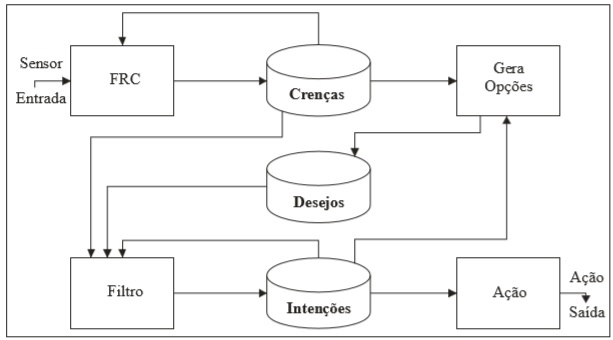
\includegraphics[width=0.9\textwidth]{images/bdiGenerica.jpg}
      \caption*{Fonte: Adaptado de \cite{Bordini:2007:PMS:1197104}}
   	  \label{fig:typesAgent}
    \end{figure}

\blindtext

\begin{figure}[h!]
  %Sempre manter mesmo valor do captionsetup com o width do \includegraphics, para assim manter o mesmo alinhamento
    \centering
    \captionsetup{width=0.6\textwidth}
    \caption{UTFPR - Campus Ponta Grossa}
    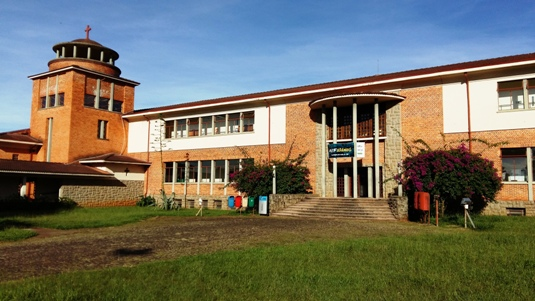
\includegraphics[width=0.6\textwidth]{images/fachada-utfpr.jpg}
    \caption*{Fonte: Sítio UTFPR (2010)}
   	\label{fig:utfpr}
\end{figure}



%Maiores informacoes Apendice e Anexo - "Leia" o README!

% \cftaddtitleline{toc}{chapter}{REFERÊNCIAS}{\pageref{ch:bib}}
\renewcommand{\bibsection}{%
	\chapter*{\bibname}
	\bibmark
	\ifnobibintoc\else
	\phantomsection
	\addcontentsline{toc}{chapter}{\hspace{-2cm}\texorpdfstring{\MakeTextUppercase{\bibname}}{\bibname}}
	\fi
	\prebibhook
}

\cftaddtitleline{toc}{chapter}{\nameref{ch:apendiceA}}{\pageref{ch:apendiceA}}
\cftaddtitleline{toc}{chapter}{\nameref{ch:anexoA}}{\pageref{ch:anexoA}}


\bibliography{ref_modeloDAINF}
\label{ch:bib}

\chapter*{APÊNDICE A - Permissão de direito autoral}
\label{ch:apendiceA}
  \blindtext

\chapter*{ANEXO A - Protótipo}
\label{ch:anexoA}
  \blindtext

\end{document}
